\renewcommand\thechapter{c2.14a}
\lab{AC circuits}\label{lab:ac-circuits}

\section*{About this lab}

\covid\ 
It is intended to be used around the 14th week in Physics 222.

\apparatus
\equip{banana plug cables (8, soldered by the student)}
\equip{USB oscilloscope (Hantek)}
\equip{assorted capacitors, 10-100 nF}
\equip{several resistors, 10-100 $\Omega$}
\equip{alligator clips (10)}
\equip{two hand-made coils}

\begin{goals}

\item[] Observe the resonance of an LRC circuit.

\item[] Determine the indunctance of a hand-made inductor.
\end{goals}

\introduction

Earlier in the semester, for lab \ref{lab:dipole-and-superposition}, you 
made a solenoid out of about 200 turns of magnet wire. The idea of this
lab is to use this solenoid as the inductor of an LRC circuit, observe
the circuit's resonance, measure the resonant frequency, and use this
to determine the inductance of the coil.

\section*{Preparation}

If you have only made one coil so far, you will need to make a second one
for this lab. Another one of the same type will work well.

While working on this lab, I found it convenient to organize my resistors
and capcitors in an egg carton.

Use the result of problem 13-10 in Fields and Circuits to estimate the
inductance of your coil. We don't expect this estimate to be incredibly
exact, because it's an approximation for a long solenoid, whereas the
one you've made is probably more short and stubby.

\section*{Setup}

The first figure shows a simplified and idealized version of how we could
do this experiment.

\fig{em-ac-resonance-covid}

We would have a function generator to create a sinusoidally oscillating
voltage and drive the LRC circuit near its resonant frequency. A separate
oscilloscope would measure the voltage across one of the components, such as
the capacitor, which is a measure of the response.\footnote{In principle, we
could get a measure of the response by measuring the voltage across any one
of the three components. But for a given $Q$, the voltage across the inductor or
capacitor is greater by a factor of $Q$ than the voltage across the resistor.}
Both the scope and the function generator need to be grounded, so we would
make sure to connect both grounds to the same place.

Even in this ideal world, there are things that can go wrong. The figure
below shows an example. If it weren't for the grounds, this would be
fine. But because the two grounds are connected to different spots in
the circuit, there is effectively a short in parallel with the inductor.
The inductor has been bypassed, and this is effectively an RC circuit.

\fig{em-ac-resonance-wrong-covid}

Even worse is the situation shown below. Here we have effectively shorted
across the outputs of the sine wave generator. This could burn out the
equipment.

\fig{em-ac-resonance-wrong-covid-2}

The actual setup for this lab is shown below. Instead of a specialized
sine wave generator, we will use the calibration output of the scope.
We have two separate circuits: a driving, or primary circuit on the left,
and a resonating LRC circuit on the right. The primary coil produces an
oscillating magnetic field, and the changing magnetic field induces
a curly electric field, which results in voltage difference across
the secondary coil, as in lab \ref{lab:covid-electromagnetism}.

\fig{em-ac-isolated-covid}

The benefit of this extra complication is that we now have an air gap
isolating the two circuits, and this makes us much less likely to destroy
the equipment inadvertently by hooking up grounds to the wrong places.
This isolation is, however, only partial. The calibration output of the
scope, in the primary circuit, is actually part of the same device as the
oscilloscope attached to the secondary circuit. They share the same ground,
which is also the same ground as the USB ground on the computer or phone that
you're using for the scope's user interface. Therefore there is still some
risk of burning our your scope, or even your computer, if you hook things
up wrong, but the risk is much reduced.

A resistor is shown in the schematic for the primary circuit.  This is
a standard type of precaution in order to protect against too much
current flowing in the primary circuit and burning out your scope.
After some investigation, I found that such a resistor seemed to be
present internally in the scope, so you don't need to add your own
resistor externally.

The presence of this resistor limits the current in
the primary circuit to on the order of a few milliamps, which is both good
and bad. It's good because it fulfills its purpose of protecting the scope,
and also protects you against the hazards of working with an inductive
circuit, which can give you a nasty shock if the current is amps rather
than milliamps. It's bad because it makes the signals in this circuit fairly
weak, so that you need to optimize the conditions in order to see anything.

The calibration output of the scope
supplies a square-wave voltage rather than a sine wave. To understand
what effect this has, we can use the fact that a square wave can be
approximated by a sum of the form
$\raisebox{-.2\height}{\includegraphics{../figs/eqn-wave1}}
+\frac{1}{3}\raisebox{-.2\height}{\includegraphics{../figs/eqn-wave3}}
+\frac{1}{5}\raisebox{-.2\height}{\includegraphics{../figs/eqn-wave5}}
+\ldots$ If you want to see this for yourself, try getting in the
graphing utility at desmos.com and telling it to graph the function
$\sin x+\left(\frac{1}{3}\right)\sin(3x)+\left(\frac{1}{5}\right)\sin(5x)$
(the extra parentheses being necessary because computers aren't good
at disambiguating their input like humans do). When I did that, here's
what my graph looked like:

\fig{covid-desmos-square-wave}

By adding more terms to the sum according to the obvious pattern of
odd numbers, you should find that you can get a better and better
approximation to a square wave. This is called Fourier analysis.
So the upshot is that using a square wave
rather than a sine wave actually doesn't matter much for this lab.
If you set the scope's calibration output to give a square wave
with some frequency $f$ such as 20 kHz, it is effectively a 20 kHz
sine wave superimposed with a $3f$ sine wave, a $5f$, and so on. But our LRC circuit's resonance peak is fairly narrow, so if
we have it tuned in pretty close to 20 kHz, then the other frequencies
simply won't produce any response.\footnote{I also found empirically that
the \emph{primary} coil made out of this magnet wire seemed to have nonideal behavior
that made it not respond very much at all to frequencies above about
100 kHz. I think this is because of stray capacitance between the adjacent
loops of wire, which makes the coil act like an inductor in parallel to
a capacitor.}

Ideally we would measure the response of the LRC circuit when we
varied the frequency, and by turning a knob we would get the frequency
that mazimized the response. This would be the resonant frequency,
which we could then use in order to determine our unknown inductance.
Actually, the frequency of the calibration output can be controlled in
the software, but not continuously; we have a discrete set of choices,
such as 10, 20, and 50 kHz. Therefore we will vary the capacitance in
order to maximize the response, i.e., we tune the oscillator to resonate
with the driver, rather than the other way around.

\section*{Designing the LRC circuit}

You may need to vary the design somewhat based on the parameters of the secondary coil you're
working with, but the setup used in the video used  a frequency of 20 kHz
and a 47 ohm resistor in the LRC (secondary) circuit. Here is the thought
process I went through in designing my circuit. I estimated the inductance
of my coil, and I set a goal of making a circuit with $Q\approx 5$.
I wanted $Q$ to be high enough so that I
would only let through the lowest frequency in the Fourier series, but
not so high that I would have difficulty tuning well enough to locate the
resonance.  The resonant frequency depends on $L$ and $C$. The $Q$ is
basically related to how much energy is dissipated as heat, so a low
$R$ makes for a high $Q$. However, $Q$ does also depend on $L$ and $C$;
the relation is $Q=R\sqrt{L/C}$. I picked one of the frequencies that
the square-wave generator was capable of putting out, found the value of
$C$ that would give me that resonant frequency (using my rough estimate of $L$),
and then determined what value of $R$ would give me the desired value of
$Q$. I initially came up with designs using relatively low frequencies, and I found that $R$
then had to be an unrealistically low value, smaller than the internal
resistance of the magnet wire I had used to wind my secondary coil.
I then played with higher values of the frequency until I got a value of 20 kHz,
which didn't require an unreasonably high $R$.

\section*{Observations}

\labpart{Determination of the inductance}

Build the driving circuit. The introductory video has some ideas on how to
make the necessary connection conveniently.
Use the ground clip on the scope's probe to complete the circuit.
This is not designed to be a current-carrying connection, but the
currents we will use are fairly small.

Build the secondary circuit, and connect the probe to the scope,
being careful, as discussed above, not to create a short. The ceramic
disk capacitors we're using are small, so there is not enough room
on them to print their values in an obvious notation. They are labeled
with numbers like 683, which is to be interpreted as $68\times10^3\ \zu{pF}$,
or 68 nF. They are nonpolar capacitors.

If your estimate of the coil's inductance was fairly good, then you
may see a clear response right away, as in the video. For example,
if your $Q$ is 5, then you will need to be within about 20\% of
the right frequency in order to lie inside the FWHM of the resonance.
If you think you're seeing the resonance, verify this as shown
in the video by changing the distance between the primary and
secondary coils.

If you aren't initially close enough to resonance
to see any response, vary the capacitance by a small amount. This
can be done either by swapping in a different capacitor or by
combining capacitors. Doing this in parallel, as shown in the video,
is pretty convenient. For example, if your initial guess for the
capacitance was 68 nF, and you want to try increasing it a little,
then putting a 10 nF capacitor in parallel with it would increase
the capacitance to 78 nF.

Once you've found the resonance, take data with several different
capacitances and try to find which capacitance comes closest to
maximizing the response. For this purpose, I used the mV$\sim$ number
displayed in the OpenHantek software at the bottom of the screen.
For example, I obtained a response of 3.6 mV with 43 nF,
5.0 mV with 47 nF, and 4 mV with 57 nF, which suggested that I
had the resonance tuned in pretty well with the intermediate
value.\footnote{This was with my initial setup, which gave pretty weak
signals. Your amplitudes should be an order of magnitude greater,
as shown in the video.}

\labpart{Response to a kick, measurement of $Q$}

Change the frequency of the calibration output's square wave to something about an order
of magnitude lower than the resonant frequency, such as 1 kHz. Zoom in and out using the
time base so you can see what is going on. What you are seeing here is essentially the
\emph{free} response of the oscillator rather than its driven response. The period of the square wave is
so long that we're essentially kicking the circuit, then waiting a long time for it to settle down,
and then kicking it again in the opposite direction. People refer to this as ``ringing''
or the ``impulse response'' of the circuit.

\fig{em-ac-impulse}

Use this setup to measure the $Q$ of your circuit. The amplitude of the decaying oscillations
after $n$ cycles dies off exponentially, as $A_n/A_0=e^{-kn}$, where the definition of $Q$
gives $k=\pi/Q$.

\labpart{Fine tuning (optional)}

The purpose of this part of the lab is to determine your inductance more precisely.
Change the frequency back to the original value.
To tune in the resonance more precisely, reduce the resistance
in the LRC circuit to 1/2 or 1/3 of its previous value, which increases
the $Q$ of the circuit by the inverse of this factor. If you already had the resonance
tuned in very precisely, then the response of the circuit should increase by the
same factor as the one by which you increased $Q$. If it doesn't, then you can now
touch up the value of $C$ by a small amount in order to tune it in. This fine-tuning
should allow you to determine the resonant value of $C$ much more precisely, because
with the higher $Q$, the resonance peak is now much narrower.

\labpart{Predicting and testing a change in resonant frequency (optional)}

Look at the list of frequencies in the menu of choices that the scope's calibration
output can provide. Pick the next one either up or down on the list, and predict what
values of $C$ and $R$ you would need in order to make the circuit resonate at that frequency,
while keeping $Q$ the same as in part A (not the larger $Q$ from part B, which makes the
resonance harder to tune in).
Test your prediction.

\labpart{Insanity (optional)}

Go back to the original setup from part A, using the original values of $f$ and $R$.
Now see what happens when you make the
capacitance many times smaller, without changing $R$. Try decreasing $C$ by a factor of 10 to 20.
You should see a waveform that is not a sine wave. Try to figure out why
you're seeing what you're seeing. Take into account the fact that changing $C$
has an effect on both the resonant frequency and $Q$.


\analysis

Determine the inductance of your inductor, with propagation of errors, and compare
with your estimate.

Determine the $Q$ from the measurement of the impulse response, and compare with theory.
